\section{要件と機能の抽出}
以下に要件を整理する.
\begin{itemize}
\item IoT機器への設定が簡略化されること
\item IoT機器が接続されるネットワークの違いによる影響を受けないこと
\item 監視サーバ上の論理的な機器と監視対象である物理的な機器との対応がわかりやすいこと
\end{itemize}

上記要件から,次のような機能を抽出した.
\begin{itemize}
\item 機器からの通知による監視情報の収集
\item 監視サーバにて機器IDとURLの対応を管理することで,監視対象機器を特定
\item 機器のIDを機器本体に掲示することで,外部からわかりやすくすること
\end{itemize}


\section{提案サービスの構成}
提案サービスは図\ref{fig:blockdiagram}のように,IoT機器上で動作するエージェントプログラム,監視サーバ上で動作するエージェントプログラム用インターフェース,機器状態データベース,機器情報データベース,可視化アプリケーションから構成されている.
\begin{figure}[htbp]
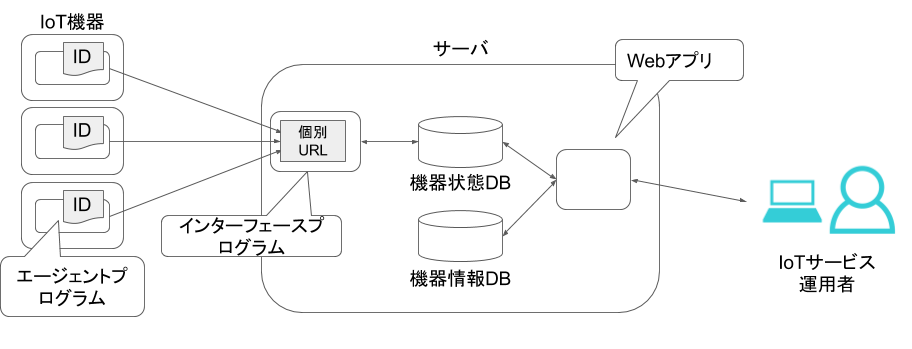
\includegraphics[width=16cm]{images/prop_diag.png}
\caption{サービス構成図}
\label{fig:blockdiagram}
\end{figure}
エージェントプログラムは,設定により与えられた機器追加用トークンを監視サーバに送信し,重複無い機器IDを取得する他,定期的に監視サーバに対して,ネットワークの状態や稼動状態を通知する.
エージェントプログラム用インターフェースは,エージェントプログラムから送信された機器追加用トークンの整合性を確認し,機器IDの発行,データベースへの登録を行う.
また,エージェントプログラムから送信されたネットワークの状態や稼動状態をデータベースへ書き込む.
機器状態データベースは,機器の状態を蓄積するために使用し,機器情報データベースは,ユーザと機器IDを結びつけ,機器に関する情報を記憶するために用いる.
可視化アプリケーションは,各データベースと連携し,機器追加用トークンの発行や,ユーザ管理,機器状態の可視化を行う.
ユーザは可視化アプリケーションへブラウザからアクセスすることで,本サービスを利用する.

\section{エージェントプログラムの設計と実装}
エージェントプログラムは,IoT機器上で動作し,IDの取得機能と,定期的な状態の通知機能を持つ.
IDの取得機能とは,ユーザから設定されたトークンを監視サーバへ送信し,機器固有のIDを取得・設定を行う機能である.
定期的な状態の通知機能とは,1分毎にネットワークの状態,機器の状態を送信する機能である.
ネットワークの状態とは,IoT機器から監視サーバへの到達性であり,「監視サーバへ接続できなかった回数」の事とする.
また,機器の動作状態とは,エージェントプログラムがサーバへネットワークの状態を通知できているかどうかであり,通知できている場合は「異常なし」と判断する.
過去のいつの時点で通信が途切れ,いつの時点で通知不能になったのか,判断するために,「過去にサーバへ接続できなかった回数」も合わせて送ることとした.

動作の流れとしては,図のようになる.
\begin{figure}[htbp]
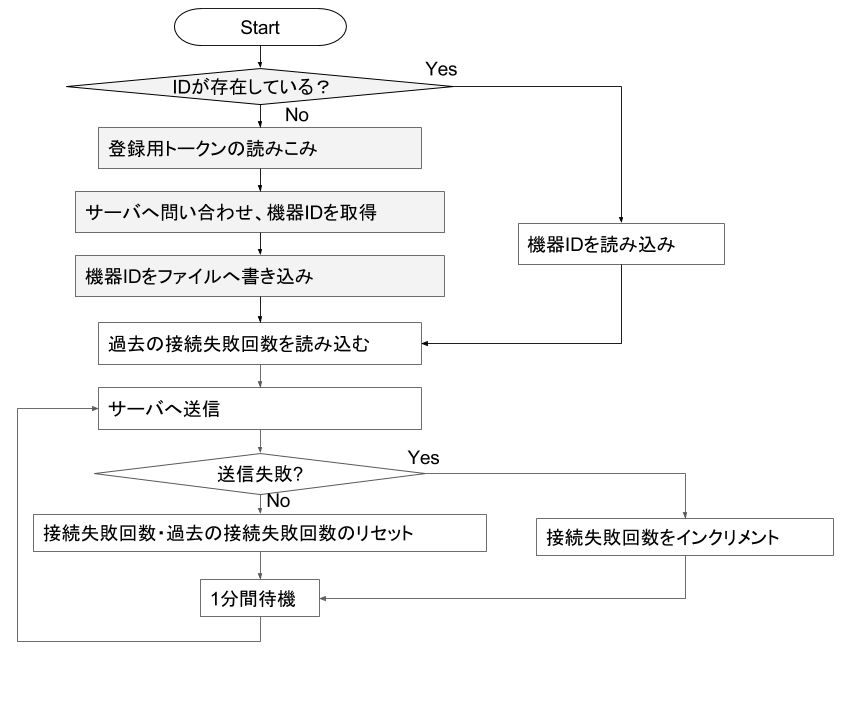
\includegraphics[width=16cm]{images/agent_flow.png}
\caption{エージェントプログラムの動作}
\label{fig:agent_flow}
\end{figure}
まず,IoT機器はユーザより設定されたトークンを監視サーバへ送信し,個別のIDを取得する.
このIDを自身へ設定しなおし,1分おきに監視サーバのIDと紐付いたURLに対して「過去にサーバへ接続できなかった回数」,「現在サーバへ接続出来なかった回数」を送信する.
「過去にサーバへ接続できなかった回数」及び「現在サーバへ接続できなかった回数は,サーバへの接続ができた時点で初期状態(0回)に戻る.

実装としては,対象となるIoT機器をRaspberryPiと仮定し開発した.
エージェントプログラムは,汎用性を高めるため,シェルスクリプトで作成した.
監視サーバへの通信には,セキュリティの設定の有無(ネットワークの多様性)を考慮し,httpsを用いる.

\section{エージェントプログラム用インターフェースの設計}
エージェントプログラム用インターフェースは,監視サーバ上で動作するプログラムで,トークンの検証機能,IDの発行機能,登録機能,機器状態の受け付け機能を持つ.
トークンの検証機能とは,IoT機器から送信されたトークンの整合性を検証する機能である.
トークンの整合性とは,トークンに紐付いたユーザが現在機器の追加を許可しているかである.
IDの発行機能とは,機器に対し,重複のないIDを発行する機能である.
登録機能とは,可視化アプリケーションへ,機器とユーザの関係を登録する機能である.
機器状態の受け付け機能とは,IoT機器から送信された機器状態等から,過去のどの時点でネットワークから切断されたのか等を逆算し,機器状態データベースへ書き込みむ機能である.

図\ref{interface_flow}は,エージェントプログラムからトークンが送られてきた場合の動作である.
\begin{figure}[htbp]
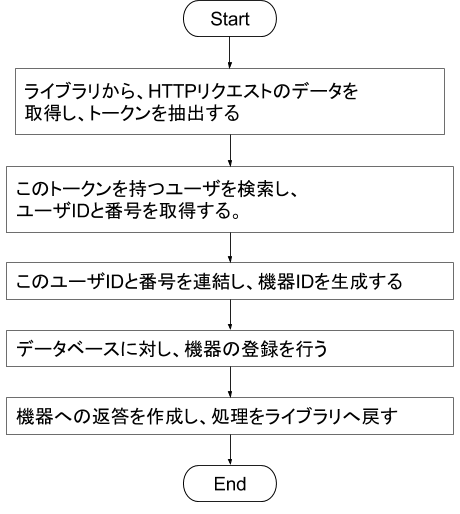
\includegraphics[width=16cm]{images/interface_flow.png}
\caption{エージェントプログラム用インターフェースの動作(機器から登録用トークンが送られてきた場合)}
\label{fig:interface_flow}
\end{figure}
IoT機器から,トークンが送られてきた場合,インターフェースは次のような動作を行う.
\begin{enumerate}
\item トークンの整合性の確認
\item ユーザ情報の取得
\item 機器IDの生成
\item 機器情報データベースへ関係を格納(登録)
\item 機器に対し,機器IDを返信
\end{enumerate}

図\ref{interface_flow2}は,エージェントプログラムから機器の状態が通知されてきた場合の動作である.
\begin{figure}[htbp]
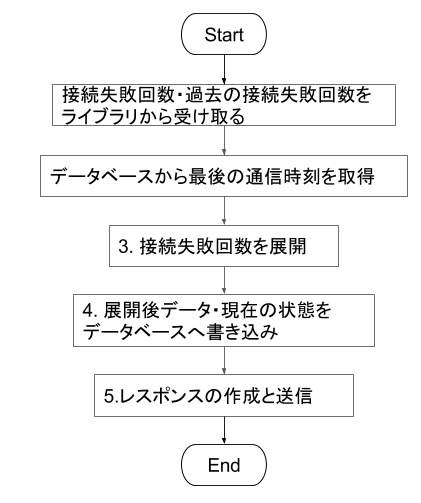
\includegraphics[width=8cm]{images/interface_flow2.png}
\caption{エージェントプログラム用インターフェースの動作(機器からの状態の通知があった際)}
\label{fig:interface_flow2}
\end{figure}

また,IoT機器から機器の状態が送られてきた場合は,次のような動作を行う.
\begin{enumerate}
\item 機器IDとURLの合致を確認
\item 過去にサーバへ接続できなかった回数と,データベース上の最後の通信の記録から,通知不能になった時刻の推測
\item 現在サーバへ接続出来なかった回数と,現在時刻から,通知可能になった時刻の推測
\item 機器状態データベースに対し,通知不能になった時刻と,通知可能になった時刻,現在時刻の3時点に対し,状態の変化を書き込む
\item 現在時刻と受理した旨を返信
\end{enumerate}

実装としては,Python3を用い,Falconと呼ばれるWebAPIの作成に特化したライブラリを使用した.
機器IDは,トークンと乱数を,sha256と呼ばれるハッシュアルゴリズムを使用してハッシュ化した物を使用する.
可視化アプリケーションへの登録は,機器情報データベースへの書き込みをもって,登録とすることとした.
このプログラムを用いて,エージェントプログラムと通信を行うために,次のようなURLを定義した.
\begin{itemize}
	\item GET /deviceid
	\item POST /<deviceid>
\end{itemize}
先頭のGET・POSTは,HTTPリクエストを表す.
また,<deviceid>は,各機器の機器IDを表す.

\section{エージェントプログラムとエージェントプログラム用インターフェース間の通信}
エージェントプログラムとエージェントプログラム用インターフェース間の通信には,HTTPSを用いる.
機器IDの取得/発行・登録時は図\ref{fig:inter_program_regist}のような動作をし,機器状態の通知/監視の際は,図\ref{fig:inter_program_monit}のような動作をする.
\begin{figure}[htbp]
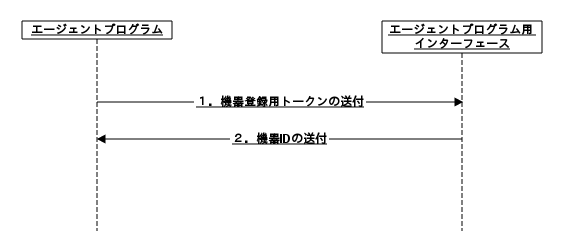
\includegraphics[width=8cm]{images/inter_program_regist.png}
\caption{機器IDの取得/発行・登録時の通信}
\label{fig:inter_program_regist}
\end{figure}
\begin{figure}[htbp]
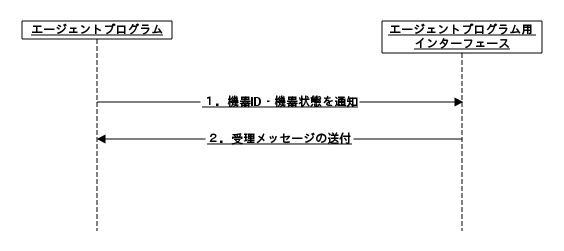
\includegraphics[width=8cm]{images/inter_program_monit.png}
\caption{機器状態の通知/監視時の通信}
\label{fig:inter_program_monit}
\end{figure}

各通信の書式はJavaScript Object Notation(JSON)という形式を用いる.
トークンを「xxxxxxxx」,機器IDを「yyyyyyyy」,過去にサーバへ接続できなかった回数と現在サーバへ接続できなかった回数をそれぞれ「pppp」・「qqqq」とすると,図中の各通信は次のようなメッセージとなる.
\begin{enumerate}
\item GET /deviceid\\
	\{ "token":"xxxxxxxx" \}
\item \{ "deviceid":"yyyyyyyy" \}
\item POST /yyyyyyyy\\
	\{ "past":"pppp", "now":"qqqq" \}
\item \{ "stat": "OK" \}
\end{enumerate}
また,トークンが不正であった場合や,デバイスIDが存在しない場合等は,サーバはデバイスに対して,HTTP Not Found(404)を送信する.


\section{機器状態データベースの設計}
機器状態データベースは,機器ごとに機器IDと同一の名前のテーブルを作成し,機器状態を管理する.
この機器IDと同一の名前を持つテーブルを機器状態管理テーブルとする.
この機器状態管理テーブルは,表\ref{tab:devstat}のような構造を持つ.
\begin{table}[htb]
\begin{center}
\caption{機器状態管理テーブル}
\label{tab:devstat}
\begin{tabular}{|l|l|l|} \hline
論理フィールド名 & 物理フィールド名 & 型 \\ \hline \hline
時刻 & time & time \\ \hline
状態 & stat & string \\ \hline
\end{tabular}
\end{center}
\end{table}

データベースはInfluxdbを利用した.
InfluxDBでは,時刻を主キー(index)として扱うので,このような構造になっている.
状態には,OK・NCが入り,OKは機器に異常が無かったこと,NCは,機器に異常は無かったがサーバーへ到達できなかった事を表す.
また,各テーブルはエージェントプログラム用インターフェースが自動で作成し,
可視化アプリケーションから,必要に応じて参照,削除を行う.

\section{機器情報データベースの設計}
機器情報データベースは,ユーザと機器の関係を格納するために使用される.
ユーザテーブル,機器情報テーブルの2つのテーブルが有り,ユーザに関する情報と,機器に関する情報を分けて記録する.
図\ref{fig:erdiagrm}は,ユーザテーブルと機器情報テーブルの関連を表す.
\begin{figure}[htbp]
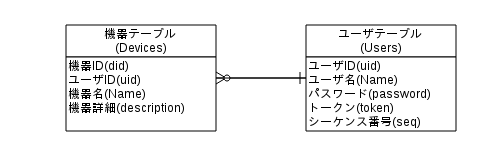
\includegraphics[width=8cm]{images/ERdiagram.png}
\caption{ユーザテーブルと機器情報テーブルの関連}
\label{fig:erdiagram}
\end{figure}
ユーザ1つに対し機器は0以上あり,機器1つに対しユーザは1つである.
ユーザテーブルと機器テーブルは,ユーザIDで紐付いている.

表\ref{tab:users}はユーザテーブルの構造を表している.
\begin{table}[htb]
\begin{center}
\caption{ユーザテーブル(Users)}
\begin{tabular}{|l|l|l|l|} \hline
論理フィールド名 & 物理フィールド名 & 型 & 制約 \\ \hline \hline
ユーザID & uid & integer & primary key \\ \hline
ユーザ名 & Name & string & unique not null \\ \hline
パスワード & password & string & not null \\ \hline
トークン & token & string & unique \\ \hline
シーケンス番号 & seq & integer & \\ \hline
\end{tabular}
\label{tab:users}
\end{center}
\end{table}
ユーザテーブルでは、サービスへのログイン時に使用するユーザ名とパスワードの他、
内部で識別のため使用するユーザID、機器登録の際に使用されるトークン、機器ID生成の為に使用されるシーケンス番号が記録される。

表\ref{tab:devices}は機器情報テーブルの構造を表している。
\begin{table}[htb]
\begin{center}
\caption{機器情報テーブル(Devices)}
\begin{tabular}{|l|l|l|l|} \hline
論理フィールド名 & 物理フィールド名 & 型 & 制約 \\ \hline \hline
ユーザID & uid & integer & foreign key primary key \\ \hline
機器ID & did & string & primary key \\ \hline
機器名 & name & strign & not null \\ \hline
機器詳細 & description & string & \\ \hline
\end{tabular}
\label{tab:users}
\end{center}
\end{table}

ユーザテーブル・機器テーブルは,エージェントプログラム用インターフェース・可視化アプリケーションから参照される.
データベースには,sqlite3を用いた.

%また,各テーブルは,次のよなSQL文にて作成した.
%SQL文入れる
%create userrs

\section{可視化アプリケーションの設計}
可視化アプリケーション次のような構造になっている.
サーバーサイドプログラムはPython3を使用し,FlaskというWebアプリケーションフレームワークを用いて作成した.
クライアントサイドプログラムは,HTML/CSS,Javascriptを使用し,Bootstrap,Jqueryというライブラリを用いた.


\section{サービス利用のイメージ}
ユーザが本サービスを利用して行うことのできる動作は,つぎのようになっている.
\subsection{機器の追加}
機器の追加は,次のような操作にて,行うことができる.
\begin{enumerate}
\item サービスにログインする
\item サービスの画面からトークンの発行を押し,トークンを保存する.
\item 各機器に対して,エージェントプログラムのインストールと,トークンの設定を行う.
\item 機器の電源を入れる
\item 機器が追加された事を確認し,機器IDを機器に対してラベル等を貼り付ける.
\item 順次他の機器に対して同様の操作を行う.
\end{enumerate}

\subsection{機器の削除}
機器の削除の利用イメージは,次のようになっている.
\begin{enumerate}
\item サービスにログインする
\item サービスの画面から,該当の機器を削除する
\item 物理的な機器の撤去を行う
\end{enumerate}



\section{実装}
時間的制約から,機器からの通知による監視のみを実装した.
付録としてソースコードを添付する.
ソースコードはgithubにも上がっている.







\begin{comment}
\section{本サービス利用のイメージ}
ユーザーは,本サービスの利用に際し,次のような動きをする.
\begin{enumerate}
\item 予め固有のIDとエージェントプログラムがインストールされた機器を買ってくる
\item ユーザは,その機器に対しサービスで利用するアプリケーションをインストールし,設置する
\item 機器は,設置後ネットワークに接続され次第,サービスへ,機器の状態の通知を行う
\end{enumerate}



\section{機器監視サービスの構成}
%(どのような要素で構成されているのか,また,それぞれの役割は何なのか)
%1.1全体構成(どのような要素で構成され,また,それぞれの役割について簡潔に述べる)
前章に述べたアイディアに基づきシステムを構築した.
システムは,エージェントプログラム,機器状態データベース,機器情報データベース,エージェントプログラム用インターフェースプログラム,Webアプリケーションサーバ,Webアプリケーションから成り立っている.
エージェントプログラムとエージェントプログラム用インターフェース,WebアプリケーションサーバとWebアプリケーションは,インターネットを介して通信しあう.
図\ref{fig:blockdiagram}は,システムのブロック図である.
\medskip

\begin{figure}[htbp]
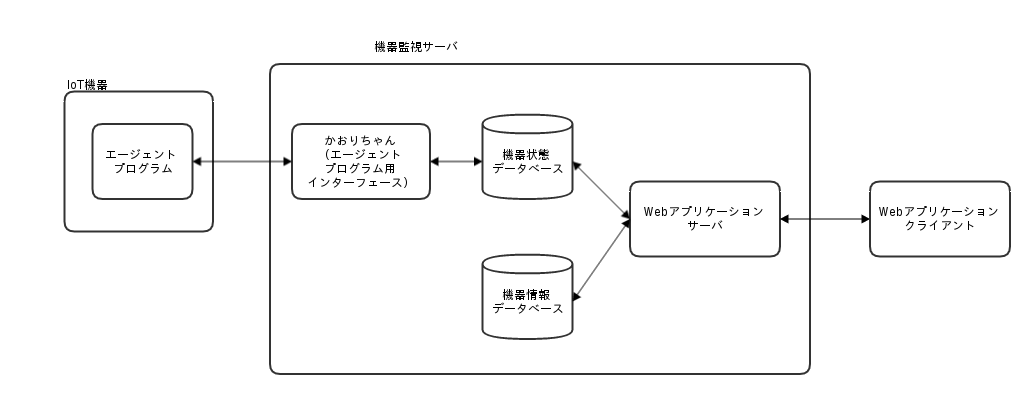
\includegraphics[width=16cm]{images/blockdiagram2.png}
\caption{システムのブロック図}
\label{fig:blockdiagram}
\end{figure}

エージェントプログラムは,IoT機器上で動作するプログラムである.
定期的に自身の状態を状態蓄積システムへ送信する役割を果たす.
定期的かつ自発的に状態を送信することで,ネットワーク環境によらない機器の監視を可能にした.
IoT機器として頻繁に使用されるRaspberryPiを想定し作成した.
%「かおりちゃん」とは,エージェントプログラム用インターフェースである.
エージェントプログラム用インターフェースは,各IoT機器上で動くエージェントプログラムから送られてきた状態を,時刻と共に機器状態データベースへ書き込む役割を果たすプログラムで,機器監視サーバー上で動作する.
機器状態データベースとは,機器の状態を時系列に沿って蓄積するデータベースである.
機器監視サーバー上で動作する.
機器情報データベースとは,機器IDや,機器名,ユーザー名を記録するデータベースである.
機器監視サーバー上で動作する.
\medskip

Webアプリケーションサーバーは,WebページやWebアプリケーション自体を配信する.
ユーザーが利用するブラウザからの要求に答え,現在の機器の状態や,機器名等を返答する.
\medskip

Webアプリケーションとは,ブラウザ上で動作するプログラムである.
ユーザーからの入力を受け付け,ユーザーへ表示する他,必要な機能を問い合わせる.
\medskip

これら各要素が連携することで,機器の監視を実現している.

\subsection{エージェントプログラム}
%(エージェントプログラムとは何なのか)
エージェントプログラムとは,IoT機器上にインストールされるプログラムである.
エージェントプログラムの役割は,定期的に送信失敗回数をエージェントプログラム用インターフェースへ報告することである.
送信失敗回数とは,ネットワークの不具合等により,機器監視サーバーへ送信されなかった報告の数である.
自発的に状態を報告するため,IoT機器にプライベートアドレスが付与されていても,状態を検知することができる.
また,HTTPを用いるため,間のネットワークにてブロックされることがない.

\subsection{エージェントプログラム用インターフェース}
エージェントプログラム用インターフェースとは,サーバー上で動くプログラムである.名前を「かおりちゃん」とした.
エージェントプログラム用インターフェースの役割は,エージェントプログラムから送信されたメッセージを受け取り,現在の時刻と正常である旨を機器状態データベースへ書き込む.
また,エージェントプログラムから送られた送信失敗回数から,IoT機器がインターネットから切断された時刻を逆算し,機器状態データベースへ書き込む事も行う.

\subsection{機器状態データベース}
%(とは何なのか)
機器状態データベースとは,サーバ上で動作するデータベースである.
各IoT機器の状態を時刻とともに記録する.
機器状態監視システムの中心にあるデータベースである.

\subsection{機器情報データベース}
機器情報データベースとは,サーバー上で動作するデータベースである.
各IoT機器の機器ID,機器名,機器詳細情報,ユーザーのメールアドレスとパスワードを記録する.

\subsection{Webアプリケーションサーバ}
Webアプリケーションサーバとは,サーバ上で動作するプログラムである.
WebアプリケーションやWebページの配信,Webアプリケーションからの要求の処理などを行う.
必要に応じて,機器状態データベースと機器情報データベースへアクセスを行う.
次に,Webアプリケーションとのインターフェースを挙げ,それぞれについて説明する.
\subsubsection{ログイン機能}
Webアプリケーションから,メールアドレスとパスワードを受け取り,	機器情報データベースのユーザーテーブルと照合する.
照合した結果,ユーザー名とパスワードが合致したユーザーが存在すれば,HTTPクッキーにセッションキーをセットし,機器状態一覧ページへのリダイレクトを返す.
合致したユーザーが存在しなかった場合,エラーメッセージを返す.
\subsubsection{ログアウト機能}
Webアプリケーションに,HTTPクッキーから該当のセッションキーを削除するよう要求する.
\subsubsection{機器情報・機器状態取得機能}
ログインチェックを行った後,機器情報データベースと機器状態データベースより,全IoT機器の機器情報と機器状態を返す.
\subsubsection{機器ID生成機能}
ログインチェックを行った後,機器情報データベースに存在しない,ランダムな機器IDを返す.
\subsubsection{機器ID重複チェック機能}
ログインチェックを行った後.Webアプリケーションから機器IDを受け取る.
機器情報データベースに該当の機器IDが存在するかしないかを返信する.
\subsubsection{機器作成機能}
ログインチェックを行った後,Webアプリケーションから,機器ID,機器名,機器の詳細と,機器の作成なのか編集なのかの指示を受け取る.
機器の作成であった場合,
機器IDに重複が無いことを確認したうえで,機器情報データベースに該当のエントリを作成・機器状態データベースにメジャーメントを作成する.
作成されたか,されなかったかを返信する.
機器の編集であった場合,
機器情報データベースから,受け取った機器IDを持つものを探しだし,編集する.
編集できたか否かを返信する.
\subsubsection{機器削除機能}
ログインチェックを行った後,Webアプリケーションから,機器IDを受け取る.
機器情報データベースから,受け取った機器IDを持つものを削除する.
その後,機器状態データベースから,メジャーメントを削除する.
削除されたか否かを返信する.
\subsubsection{過去の機器状態取得機能}
ログインチェックを行った後,機器状態データベースから,全てのIoT機器の過去の状態をまとめ,返信する.

\subsection{監視アプリケーション}
Webアプリケーションとは,ユーザーのブラウザ上で動作するアプリケーションである.
ユーザーへグラフィカルインターフェースを提供する.
必要に応じて,Webアプリケーションサーバへ必要な情報を要求する.
Webアプリケーションは,3つのWebページから成り立っている.
以下に各ページとそれぞれの役割を述べる.
\begin{itemize}
	\item ログインページ\\
		正当なユーザーであることを確認するために,メールアドレスとパスワードの入力を求める.
		メールアドレスとパスワードは,Webアプリケーションサーバーへ送信される.
		図\ref{fig:ss_login}は,ログインページのスクリーンショットである.
		\begin{figure}[htbp]
		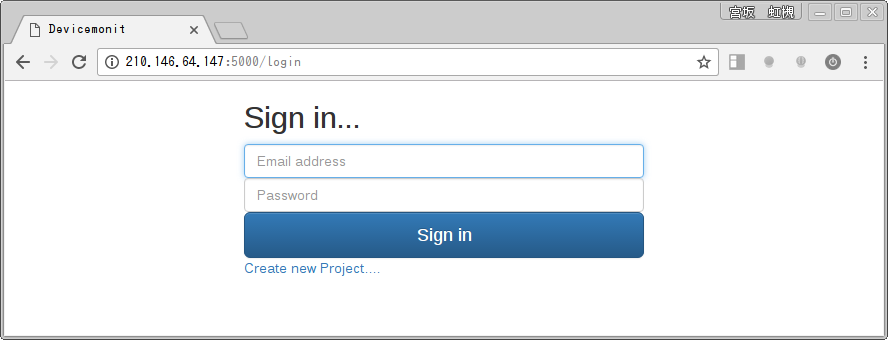
\includegraphics[width=16cm]{images/login.png}
		\caption{ログイン画面}
		\label{fig:ss_login}
		\end{figure}

	\item 機器状態一覧ページ\\
		機器状態を一覧して表示する他,機器の作成や,機器情報の編集,機器の削除等を行う事ができる.
		現在の機器の状態を取得するため,定期的にWebアプリケーションサーバと通信する.
		また,機器の作成や機器情報の編集,削除の為,Webアプリケーションサーバと通信する.

		図\ref{fig:ss_sum1}・図\ref{fig:ss_sum2}・図\ref{fig:ss_more}はこのページのスクリーンショットである.
		それぞれ,一覧表示・縮小一覧表示・詳細な情報の表示をしている.
		図\ref{fig:ss_add}・図\ref{fig:ss_mod}は,それぞれ,機器追加ダイアログ・機器情報編集ダイアログのスクリーンショットである.
		\begin{figure}[htbp]
		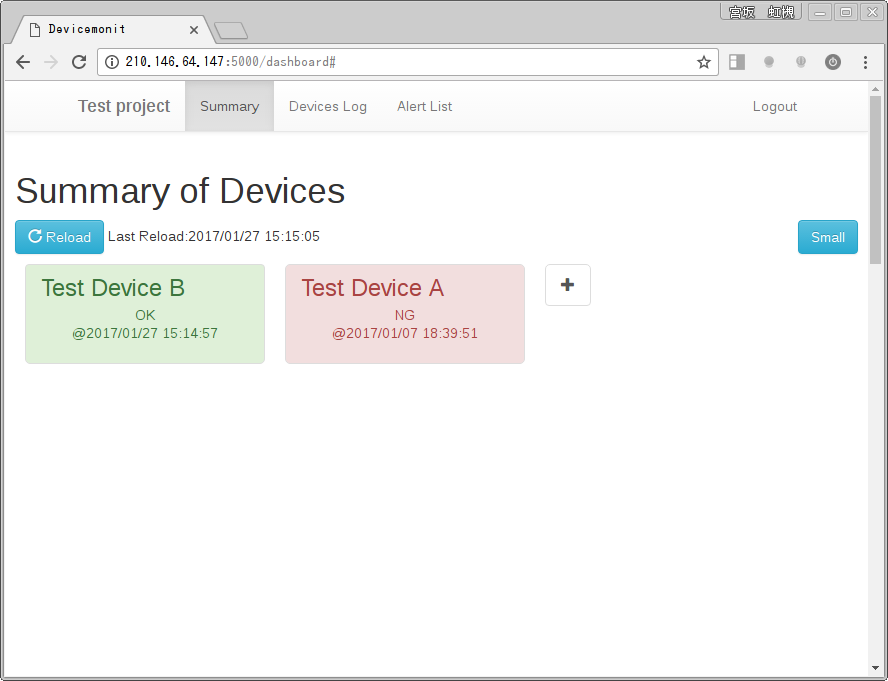
\includegraphics[width=8cm]{images/screenshot_summary1.png}
		\caption{機器状態一覧画面}
		\label{fig:ss_sum1}
		\end{figure}
		
		機器が多くなっても一覧して分かるよう,小さく表示する表示の切替機能も実装した.
		\begin{figure}[htbp]
		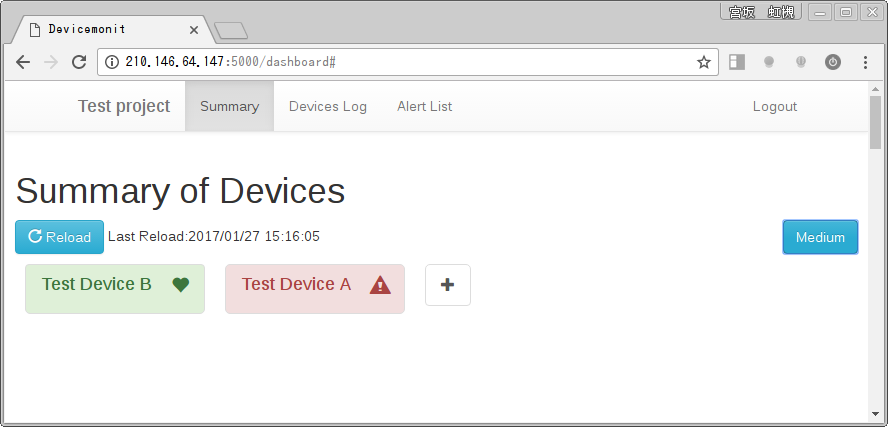
\includegraphics[width=8cm]{images/screenshot_summary2.png}
		\caption{機器状態一覧画面(小さく表示)}
		\label{fig:ss_sum2}
		\end{figure}
		
		図\ref{fig:ss_more}は,各機器の詳細を表示している様子である.
		各機器を模した図形をクリックすることで,詳細表示の切替が行える.
		\begin{figure}[htbp]
		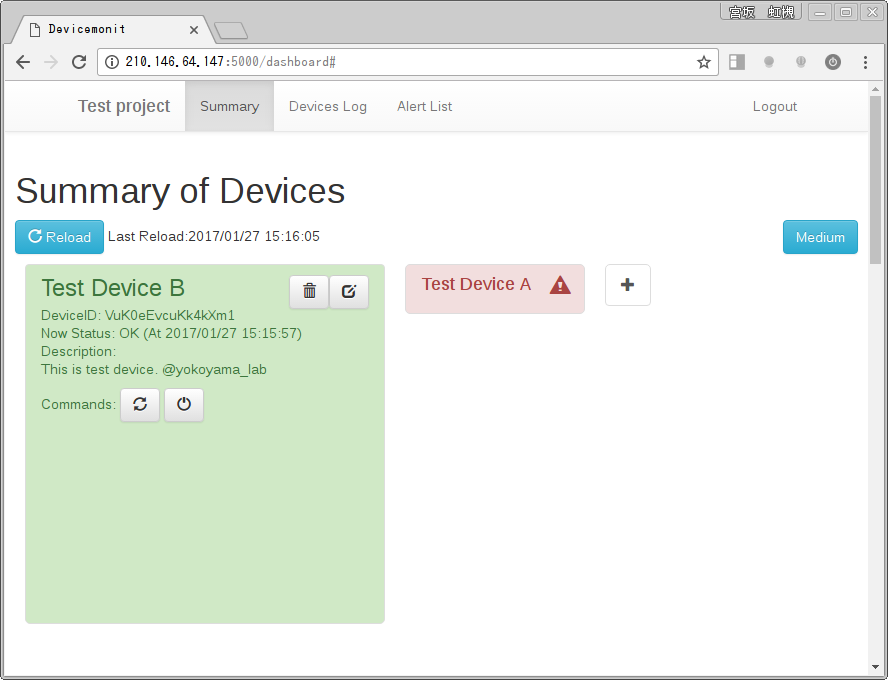
\includegraphics[width=8cm]{images/screenshot_more.png}
		\caption{機器状態詳細表示}
		\label{fig:ss_more}
		\end{figure}

		図\ref{fig:ss_add}は,新たに機器を追加する際に表示されるダイアログである.
		\begin{figure}[htbp]
		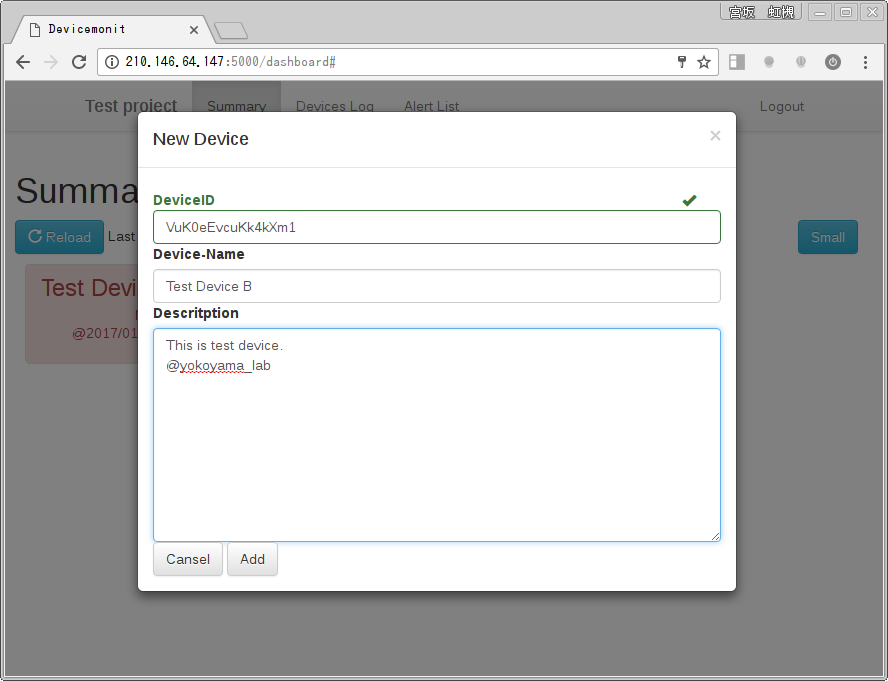
\includegraphics[width=8cm]{images/screenshot_add.png}
		\caption{機器追加ダイアログ}
		\label{fig:ss_add}
		\end{figure}

		図\ref{fig:ss_mod}は,機器の詳細情報を編集する際の画面である.
		\begin{figure}[htbp]
		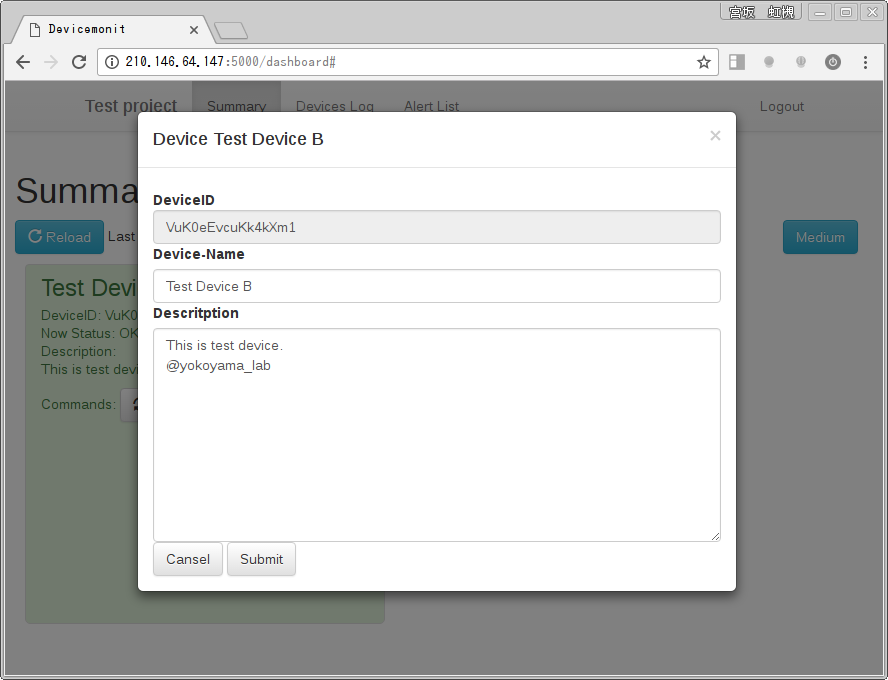
\includegraphics[width=8cm]{images/screenshot_mod.png}
		\caption{機器情報編集ダイアログ}
		\label{fig:ss_mod}
		\end{figure}


	\item 過去の機器状態一覧ページ\\
		過去の機器状態を時刻と共に整理し,一覧表示するページである.
		現在の機器の状態を取得するため,定期的にWebアプリケーションサーバと通信をする.
		図\ref{fig:ss_logs}は,スクリーンショットである.
		\begin{figure}[htbp]
		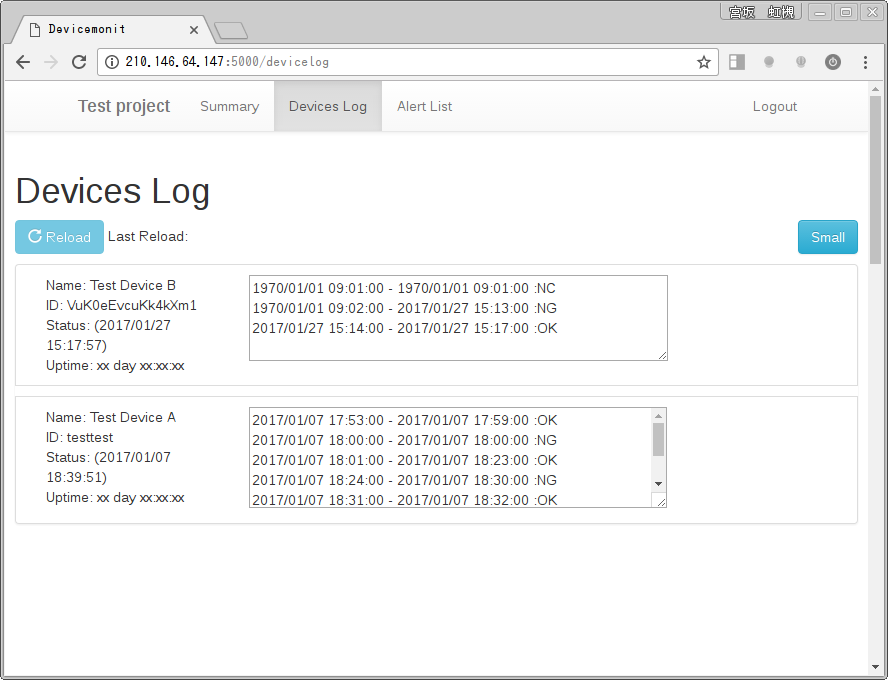
\includegraphics[width=8cm]{images/screenshot_logs.png}
		\caption{過去の状態表示ページ}
		\label{fig:ss_logs}
		\end{figure}

\end{itemize}
\section{機器監視サービスの実装}
\subsection{エージェントプログラムの実装}
エージェントプログラムの役割は,送信失敗回数を定期的にIoT機器監視サーバーに送信することにある.
約1分おきに,現在の送信失敗回数と過去の送信失敗回数を,エージェントプログラム用インターフェースへ送信する.
どのようなLinux環境でも動作することを考え,Shellスクリプトにて実装した.
\medskip

エージェントプログラムの動作は次のようになる.
\begin{enumerate}
\item エージェントプログラムが起動されると,まず過去に記録された送信失敗回数を読み出す.
\item エージェントプログラム用インターフェースに対し,過去に記録された送信失敗回数と,現在の送信失敗回数を送信する.%そうか!送信失敗回数は2種類ある!この説明をせねば!
\item サーバーから応答があった場合,過去に記録された送信失敗回数と,現在の送信失敗回数をクリアしする.\\
サーバーから応答がない場合,現在の送信失敗回数をインクリメントする.
\item 1分間スリープし,再び2から繰り返す.
\end{enumerate}


\subsection{エージェントプログラム用インターフェースの実装}
エージェントプログラム用インターフェースの役割は,エージェントプログラムから送信失敗回数を受け取り,時刻と正常である旨を機器状態データベースへ書き込むこと,
また,エージェントプログラムから送られた送信失敗回数から,インターネットより切断された時刻を逆算し,機器状態データベースへ書き込む事である.
Falconと呼ばれるAPIの作成に特化したフレームワークを使用し,Pythonにて実装した.
また,機器状態データベースへの書き込みには,InfluxDBClientというライブラリを使用した.

\subsection{機器情報データベース}
機器情報データベースの役割は,機器の名前,機器の詳細説明,機器ID,ユーザーID,ログイン用メールアドレスとパスワードを記録し保持する事である.
ユーザIDとは,システムにてユーザーを識別するための識別子である.
機器IDは,システムにてIoT機器識別するための識別子である.
機器情報データベースには,SQLitei3を用いた.
機器情報データベースには,次のようなテーブルが用意されている.
\subsubsection{機器情報テーブル}
機器ID,ユーザーIDをキーとして,機器の名前,機器の詳細説明を記録し保持するテーブルである.
\begin{table}[htb]
\begin{center}
\caption{機器情報テーブル(物理名:devices)}
\begin{tabular}{|l|l|l|l|} \hline
論理フィールド名 & 物理フィールド名 & 型 & 制約\\ \hline \hline
機器ID & did & Text & Primary key \\
ユーザID & uid & Integer & Primary key \\
機器名 & name & Text &  \\
詳細説明 & description & Text &  \\ \hline
\end{tabular}
\label{tab:}
\end{center}
\end{table}

\subsubsection{ユーザーテーブル}
ユーザーIDをキーとして,ユーザー名とパスワードを記録し保持するテーブルである.
\begin{table}[htb]
\begin{center}
\caption{ユーザテーブル(物理名:User)}
\begin{tabular}{|l|l|l|l|} \hline
論理フィールド名 & 物理フィールド名 & 型 & 制約\\ \hline \hline
ユーザID & uid & Integer & Primary key, auto increment \\
メールアドレス & email & Text &  \\
パスワード & pass & Text &  \\ \hline
\end{tabular}
\label{tab:}
\end{center}
\end{table}

\subsubsection{各テーブルの関連}
図\ref{fig:erdiagram}は,各テーブルの関連を表している.
ユーザテーブルと機器情報テーブルは,ユーザIDにて関連付けられている.
ユーザは0以上の機器情報と関連付けられ,機器情報は一つのユーザーに関連付けられている.
\begin{figure}[htbp]
\begin{center}
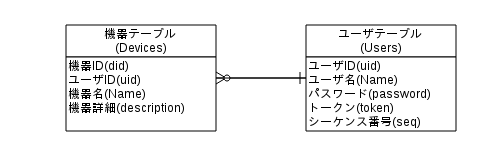
\includegraphics[width=8cm]{images/ERdiagram.png}
\caption{機器情報テーブルとユーザテーブルの関連}
\label{fig:erdiagram}
\end{center}
\end{figure}

\subsection{機器状態データベース}
機器状態データベースの役割は,機器の状態を時刻と共に記録・保持することである.
機器状態データベースには,Influxdbを用いた.
機器IDをメトリクス名(テーブル名)とし,時刻をキーとして,機器の状態を記録している.
\begin{table}[htb]
\begin{center}
\caption{}
\begin{tabular}{|l|l|l|} \hline
フィールド名 & 型 & 制約\\ \hline \hline
時刻 & Timestamp & \\
状態 & Text & \\ \hline \hline
\end{tabular}
\label{tab:}
\end{center}
\end{table}

\subsection{監視アプリケーション}
監視アプリケーションの役割は,与えられたHTTPリクエストを元に,Webページや,各種情報を返却することにある.
Flaskと呼ばれるWebアプリケーションフレームワークを用いた.Pythonを使用している.
Webサーバーアプリケーションの設計とWebアプリケーションの設計から,下記の様に実装した.
やり取り先頭に付いているGETやPOSTはHTTPメソッド,/login等はURLを示している.
図\ref{fig:diag_apps}は,サーバー上で動く監視アプリケーションとユーザのブラウザ上で動くWebアプリケーションとのやり取りを表している.
\begin{figure}[htbp]
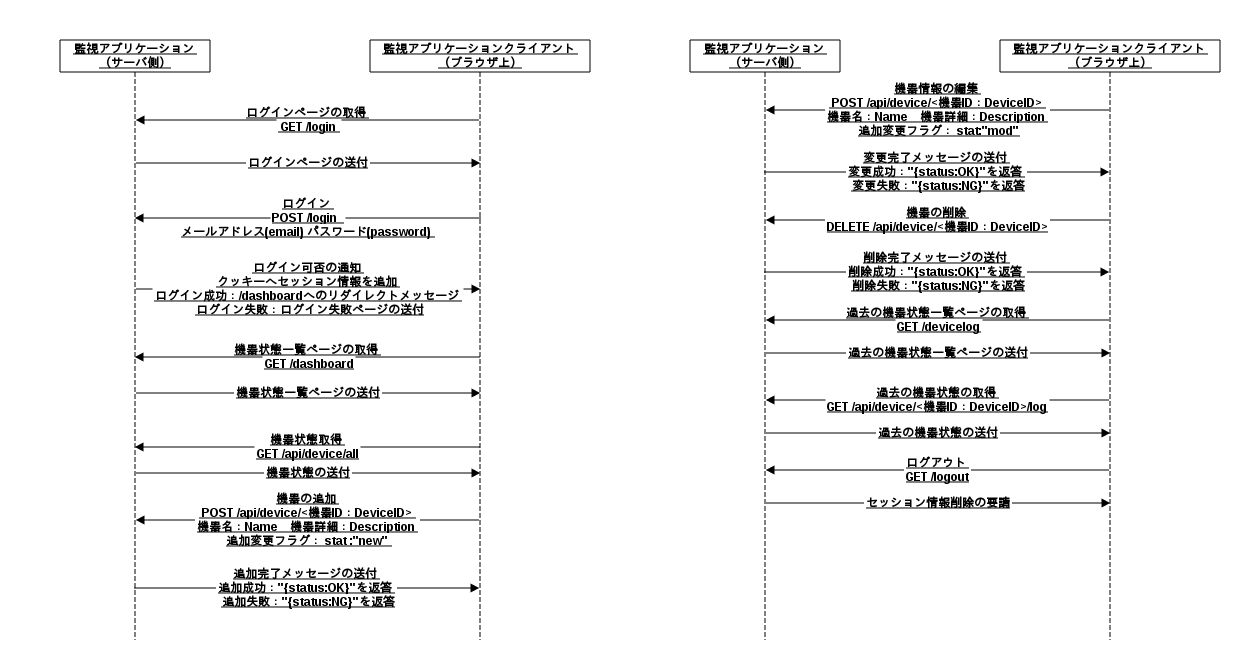
\includegraphics[width=16cm]{images/diag_apps.png}
\caption{エージェントプログラムとエージェントプログラム用インターフェースの間のメッセージシーケンス図}
\label{fig:diag_apps}
\end{figure}


\begin{description}
	\item[GET /login]\mbox{}\\
		ログインページを返す.
	\item[POST /login]\mbox{}\\
		メールアドレスとパスワードを受け取る.
		クッキーからセッションキーを探し,存在すれば既にログインしているとして,/dashboardへのリダイレクトメッセージを返す.
		データベースにメールアドレスとパスワードの組が存在するか確認し,存在した場合,セッションキーを返す.
		存在しなかった場合,ログインエラーページを返す.
	\item[GET /logout]\mbox{}\\
		セッションキーを受け取り,該当のセッションを削除する.
	\item[GET /dashboard]\mbox{}\\
		ログインチェックをし,機器状態一覧ページを返す.
	\item[GET /devicelog]\mbox{}\\
		ログインチェックをし,過去の機器状態一覧ページを返す.
	\item[GET /api/device/all]\mbox{}\\
		ログインチェックをし,現在の状態,最後にメッセージを受け取った日時,機器ID,機器名,機器詳細のデータを,JSON形式にまとめたものを返す.
	\item[GET /api/deviceID]\mbox{}\\
		ログインチェックをし,ランダムにデバイスIDを生成し,JSON形式にまとめたものを返す.
	\item[POST /api/deviceID]\mbox{}\\
		ログインチェックをし,受け取ったデバイスIDが既に存在するか確認し,その結果をJSON形式にまとめ,返す.
	\item[POST /api/device/\{DeviceID\}]\mbox{}\\
		ログインチェックをし,デバイスIDと受け取ったJSONデータから,デバイスの新規作成・編集をし,結果をJSON形式にまとめ,返す.
	\item[DELETE /api/device/\{DeviceID\}]\mbox{}\\
		ログインチェックをし,該当のデバイスIDを持つデバイスをデータベースから削除する.	
\end{description}


\subsection{Webアプリケーション}
Webアプリケーションの役割は,ユーザーインターフェースを提供することである.
Bootstrap,JQueryというライブラリを用いて作成した.HTML,CSS,Javascriptで書かれている.
定期的にWebアプリケーションサーバから状態を取得し,HTML,CSSを用いて表示する.

\subsection{エージェントプログラムとエージェントプログラム用インターフェース間の通信の実装}
%このような形式で,どんな情報を伝えているのか.
%特徴としてどのような事があるのか
エージェントプログラムとエージェントプログラム用インターフェースは,インターネットを介して,HTTPというプロトコルを用いて通信する.
エージェントプログラムとエージェントプログラム用インターフェース間の通信は次の様な形になる.
\begin{enumerate}
	\item エージェントプログラムがエージェントプログラム用インターフェースに対し,送信失敗回数を報告する.
	\item エージェントプログラム用インターフェースは,時刻と正常である旨を機器状態データベースへ送信する.
	\item 機器状態データベースより,正常に書き込んだというメッセージが返ってくる.
	\item エージェントプログラム用インターフェースは,必要に応じて送信失敗回数からインターネットから切断された時刻を逆算し,その時刻と切断されていた旨を機器状態データベースへ送信する.
	\item 機器状態データベースより,正常に書き込んだというメッセージが帰ってくる.
	\item エージェントプログラム用インターフェースは,エージェントプログラムに対し,正常に受け付けたというメッセージを返す.
\end{enumerate}
エージェントプログラムとエージェントプログラム用インターフェースの間の通信は,約1分おきに繰り返される.
\begin{figure}[htbp]
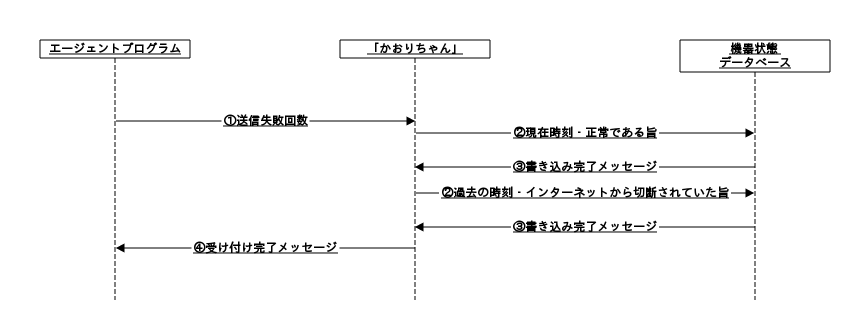
\includegraphics[width=16cm]{images/seq1.png}
\caption{エージェントプログラムとエージェントプログラム用インターフェースの間のメッセージシーケンス図}
\label{fig:blockdiagram}
\end{figure}

HTTP上でやり取りするデータの形式としては,Javascript Object Notation(JSON)という形式を用いる.
エージェントプログラムからは,次のような形式でメッセージが送られる.
\begin{lstlisting}[caption=エージェントプログラムからエージェントプログラム用インターフェースに送られるメッセージの書式,label=format1]
{"seq":<NOW>, "stat":"OK", "log":{"seq":<PAST>}}
\end{lstlisting}
<NOW> には,現在の送信失敗回数が入る.
<PAST> には,過去の送信失敗回数が入る.


また,エージェントプログラム用インターフェースからは,次のような形式で応答がある.
\begin{lstlisting}[caption=エージェントプログラム用インターフェースからエージェントプログラムへの応答の形式,label=format2]
{"stat":"OK", "time":<NOWTIME> }
\end{lstlisting}
ここで,<NOWTIME> にはサーバー側の現在時刻が入る.


\subsection{WebアプリケーションサーバとWebアプリケーション間の通信の実装}
%どのような形式で,どのような情報を伝えているのか.
WebアプリケーションサーバとWebアプリケーションは,インターネットを介し,HTTPというプロトコルを用いて通信する.
HTTP上でやり取りするデータの形式としては,Javascript Object Notation(JSON)という形式を用いる.

\section{ソースコード}
下記URLにて,ソースコードを公開している.
\url{https://github.com/miyasakakoki/devicemonit/tree/feature}

\section{サービスによる監視のイメージ}
従来は,
VPNを使用して,サーバと各IoT機器を繋ぎ,ssh等でログインすることで,監視を行っていた.
しかし,本サービスを利用することで,サービスにログインすることで監視を行うことができるようになる.


%ユーザー目線で,ユーザーは何をしてこれこれこうする みたいな.
本サービスで想定するユーザーの動きをまとめる.
\begin{itemize}
\item ユーザーがIoT機器をサービスに登録する場合
	\begin{enumerate}
	\item ユーザーは最初にサービスにログインし,機器一覧ページへ遷移する.
	\item ユーザーは機器一覧ページにある「+」ボタンを押す.すると,機器追加用ダイアログが表示される.
	\item 機器IDが既に決まっている場合は,機器ID欄を書き換える.\\
		決まっていない場合は,機器ID欄に表示されている機器IDをメモしておく.
	\item 機器名,機器詳細を入力する.
	\item 機器の追加ボタンを押し,機器一覧に追加した機器が表示されていることを確認する.
	\item ユーザーは,IoT機器へエージェントプログラムをインストールし,自動でエージェントプログラムが起動するよう設定する.
	\item ユーザーは,IoT機器をインターネットに繋ぎ,サービスの機器状態一覧ページの表示が変わったことを確認する.
	\end{enumerate}
\item ユーザーがIoT機器の情報を変更する場合
	\begin{enumerate}
	\item ユーザーは,サービスにログインし,機器一覧ページへ遷移する.
	\item 該当の機器をクリックし開く.
	\item 該当の機器の編集ボタンを押すと,機器情報編集ダイアログが表示される.
	\item 機器名,機器詳細を編集し,OKボタンを押す.
	\end{enumerate}
\item ユーザーがIoT機器を削除する場合
	\begin{enumerate}
	\item ユーザーは,サービスにログインし,機器一覧ページへ遷移する.
	\item 該当の機器をクリックし開く.
	\item 該当の機器の削除ボタンを押すと,確認ダイアログが表示されるので,OKを押す.
	\item 機器一覧ページから,機器が消えたことを確認する.
	\end{enumerate}
\item ユーザーが現在の機器の情報,機器の状態を確認する場合
	\begin{enumerate}
	\item ユーザーはサービスにログインし,機器一覧ページへ遷移する.
	\item 該当の機器をクリックし開くと,機器の情報がと,現在の状態,最後に通信があった日時等が表示される.
	\item また,機器一覧ページにて機器の背景が,緑色である場合は正常で,赤色である場合は異常である.
	\end{enumerate}
\item ユーザーが過去の機器状態を確認する場合
	\begin{enumerate}
	\item ユーザーは,サービスにログインし,機器一覧ページへ遷移する.
	\item ナビバーから過去の機器状態ページへ遷移する.
	\item すると,機器と機器の過去の状態一覧が表示されるので,該当の機器を見つけ出し,確認する.
	\end{enumerate}
\end{itemize}
\end{comment}




